% This class inherits from the LaTeX standard report class and should support
% many of the options supported by it, as well as a few extra. These extra
% options are described here.
%
% By default the document uses doublespacing, if this is unsedired, these
% options are provided:
% singlespacing, onehalfspacing, doublespacing
%
% By default the lists: table of contents, list of figures, list of tables and
% list of symbols (toc, lof, lot, los) use onehalfspacing. This can
% be overridden with the options:
% singlespacelists, onehalfspacelists, doublespacelists
% If different spacing is desired for different lists, the following macros can
% be redefined t set up the desired spacing:
% \@tocspacing, \@lofspacing, \@lotspacing, \@losspacing
% For example:
% \renewcommand*\@lofspacing\singlespacing
% Will set single spacing on the list of figures, and the remaining lists will
% use whatever was set by the class options, or the default.
%
% If the microsystems title page and signature sheet should be used:
% microsys
%
% The bibliography is single spaced by default. If this is undesired, these
% options will change the bibliography spacing:
% singlespacebib, onehalfspacebib, doublespacebib
%
% Most pages, other than the first page of a chapter or a list, or a special
% page, such as the signature sheet, have a header showing the current chapter
% name. This may be undesired, and can be removed with the option:
% nohead
%
% Page numbers are located in the bottom right corner of the page. If instead
% they should be centered, this option will do so:
% pagenumcenter
%
% This class can also be used to write a proposal. When doing so, the top level
% sectioning elements are sections rather than chapters, and the document is
% centered on the page, rather than offset for binding as the thesis is. The
% proposal formatting can be achieved with the option:
% proposal
%
% In order to create a buildable document, you first must include a lot of
% information about your school and program, much of this information can be
% automatically included by using one or more of the following options:
% ms, phd, microe, microsys, rit
%
% If using either 'microe', 'cmpe' or 'microsys', then none of the other options
% should be necessary. However, if using either the 'ms', or the 'phd' option,
% 'rit' is likely a desired option as well
%

\documentclass[microe]{ritthesis}

%%%%%%%%%%%%%%%%%%%%
%%%%% Packages %%%%%
%%%%%%%%%%%%%%%%%%%%
% Used for filler text but will almost certainly be of no use in a real thesis
\usepackage{lipsum}
% Generally you will want to use the graphicx package to display images
\usepackage{graphicx}
% You can set the graphicspath if you want to use pictures no in the same
% directory as the .tex file
%\graphicspath{{images/}}

% If subfigures or subtables are desires, the subcaption package is the
% recommended way to go. This package should not be used unless subfigures or
% subtables (or any other functionality it provides) is desired. It will not
% work if the subfig package is used.
%\usepackage{subfig}
\usepackage{subcaption}

% Use these commands to set up the author, title, and date
\author{Udita Kapoor}
% You most likely need to insert a line break or two to make the title wrap
% more evenly
\title{Introduction to Atomistic Simulation using NEMO5}
\date{Dec 19, 2018}

% You can further customize the appearance of the title and author by
% uncommenting and changing:
% \makeatletter
% \renewcommand{\thetitle}{\textbf{\large\@title}}
% \renewcommand{\theauthor}{\textsc{\@author}}
% \makeatother
% But I like small caps, so that is how I made it

% There are also a bunch of other commands that can be changed, were this not
% a masters thesis in microelectronic engineering at RIT. Those would be the
% following:
% \renewcommand*{\universityname}{Rochester Institute of Technology}
% \renewcommand*{\collegename}{Kate Gleason College of Engineering}
% \renewcommand*{\departmentname}{Department of Electrical and Microelectronic Engineering}
% \renewcommand*{\logo}{kgcoelogohoriz}
% \renewcommand*{\degreename}{Master of Science}
% \renewcommand*{\degreefield}{Microelectronic Engineering}
% Some or all of these may be set by a class option such as 'microe', 'rit', or
% 'phd' and are therefore not required in every document.

% Each of these commands can be repeated as many times as necessary
% Used to create the lines on the signature sheet. There is an optional first
% argument for each of these to specify title (the default is Dr.)
\advisor{Assistant Professor}{Sean}{Rommel}
\committee{Professor, Microelectronic Engineering}{Karl}{Hirschman}{}
\committee{Program Director, Microelectronic Engineering}{Robert}{Pearson}{}
\committee{Professor, Electrical Engineering}{James E.}{Moon}{}
\committee{Professor, Microelectronic Engineering}{Jing}{Zhang}{}
\committee{Department Head of Electrical and Microelectronic Engineering}{Sohail A.}{Dianat}{}
%\committee[Mr.]{Bystander}{Robert}{van Rosenson XXXVIII}{King of the Committee}

% If you want a second "Certified By" section
%\certifiedby[Mr.]{Bystander}{Robert}{van Rosenson XXXVIII}{King of the Committee}
%\certifiedby[Mr.]{Bystander}{Robert}{van Rosenson XXXVIII}{King of the Committee}

%\renewcommand\certificationmessage{Here you can insert a certification message. Perhaps something along the lines of ``We the undersigned committee members certify that the student has completed the requirements.'' But you should probably make it sounds better than that.}

% You can customize the signature line by redefinding the following:
% \renewcommand*\@siglinelength\linewidth
% \setlength\@siglineheight{1pt}

% This command makes testing the proposal option easier
% it should not be used in a real document
% It just redefines \chapter to be the same as \section
%\providecommand{\chapter}[1]{\section{#1}}

% Begin the document, the way you always do in LaTeX
\begin{document}
	
% This starts the pages that get roman numerals at the beginning of the
% document. Generally is the first thing in the document.
\frontmatter

% Instead of \frontmatter it is possible to do what that macro does
% manually, if more control was desired. If that is the case, uncomment and
% change, or just use the individual macros:
% \renewcommand{\frontmatter}{\pagenumbering{roman}\maketitlepage\makesignaturepage}
% Each of these commands can also be changed, but for details on that you
% should look in ritthesis.cls to see how they are defined

% The following three environments are optional and can be included in any
% order. Each of these environments has an optional argument to either include
% or suppress inclusion of the environment in the table of contents. Simply use
% either 'n' or 'y' to suppress the entry, or include the entry, in the toc.
% By default, only the abstract is included in the toc.

% The acknowledgments environment will create an acknowledgments section,
% complete with a correctly spelled title. Change the following to rename
%\renewcommand{\acknowledgmentsname}{Acknowledgments}
\begin{acknowledgments}
\lipsum[4-6]
\end{acknowledgments}

% The dedication environment will create a dedication section, change the
% following to rename
%\renewcommand{\dedicationname}{Dedication}
\begin{dedication}

\end{dedication}

% The abstract environment is very similar to the acknowledgments environment
% and is used the same. Change the following to rename
%\renewcommand{\abstractname}{Abstract}
\begin{abstract}
\lipsum[1-2]

\end{abstract}

% Makes the table of contents, list of figures, and list of tables, in that
% order. This command makes a table of contents entry for each of these lists
\makealllists

% Here you can generate a list of symbols, or a list of abbreviations, or whatever
% other custom lists you may desire. These lists are built using the longtable
% environment, and takes similar arguments
% You can change the list of symbols name by either uncommenting the following line
% and making the desired change, or by providing the optional argument to the
% listofsymbols environment
%\renewcommand{\listofsymbname}{List of Symbols}
% The first argument is column alignment options and uses the same syntax as the
% argument for the longtable environment (which is similar to the tabular environment)
% The second argument is the column headers, separated by ailgnment characters (&)
% If you want multiple extra tables, such as a table of acronyms, and a table of symbols
% you can just use this environment multiple times, with different names
\begin{listofsymbols}[List of Symbols]{lp{0.6\linewidth}r}{Term & Description & Units/Value}
$C_D^\prime$ 	& Depletion region capacitance per unit area 			& F/cm\textsuperscript{2}\\
$C_{ox}^\prime$ & Oxide capacitance per unit area 						& F/cm\textsuperscript{2}\\
$\mathcal{E}$	& Electric field 										& V/cm\\
$E_c$ 			& Energy at the conduction band edge 					& eV\\
$E_F$			& Fermi level											& eV\\
$E_g$			& Band gap energy 										& eV\\
$E_v$ 			& Energy at the valence band edge 						& eV\\
$E_x, E_y$		& Electric field normal and parallel to the gate		& V/cm\\
$\hbar$			& Reduced Planck constant 								& $6.582\times 10^{-16}$ eV$\cdot$s\\
$I_D$			& Drain current											& A\\
$J_t$			& Band to band tunneling current density 				& A/cm\textsuperscript{2}\\
$k$				& Boltzmann's constant 									& $8.617\times 10^{-5}$ eV/K\\
$m^*$			& Carrier effective mass 								& kg\\
$N_A$			& Acceptor concentration 								& cm\textsuperscript{-3}\\
$N_c$			& Effective density of states in the conduction band 	& cm\textsuperscript{-3}\\
$n_i$ 			& Intrinsic carrier concentration						& cm\textsuperscript{-3}\\
$q$				& Elementary charge  									& $1.602\times 10^{-19}$ C\\
$S$ 			& Subthreshold swing 									& V/dec\\
$T$				& Temperature											& K\\
$V_{DS}$		& Drain--Source voltage 								& V\\
$V_{eff}$		& Effective reverse bias voltage						& V\\
$V_{FB}$ 		& Flatband voltage 										& V\\
$V_G$ 			& Gate voltage 											& V\\
$\epsilon_s$	& Permittivity of a semiconductor 						& F/cm\\
$\mu_n, \mu_p$  & Mobility of electrons and holes respectively 			& cm/V$\cdot$s\\
$\Psi_s$ 		& Surface potential										& V\\
\end{listofsymbols}

% The \mainmatter macro starts the main matter. This starts arabic numbering,
% and adds a header (except on the first page of a chapter).
\mainmatter

% This class uses the fancyhdr package to build the headers. You could probably
% customize the headers by changing the plain page style, as well as the fancy
% page style. There is no guarantee anything you do works though. (In fact,
% there isn't a guarantee anything in ritthesis.cls works.)

% Likewise, the chapter and section headers are formatted using the titlesec
% package. You should be able to customize them by using that package's
% commands, specifically \titleformat

% Begin new chapters the way you always do it LaTeX
\chapter{Introduction and Motivation}

\section{Background}
\section{Overview of TMD TFETS}
\section{Current research state of TMD devices}
\section{Thesis Outline}

\chapter{Theory of Atomistic Modeling}
\section{Tight Binding Models for Material Characterization}
\subsection{DFT}
\subsection{LDA}
\subsection{GGA-PBE}
\subsection{HSE06}

\section{Charge Transport Model Theory}
\subsection{QTBM}
\subsection{NEGF/RGF}
\section{Conclusion}

% Same goes for sections

% Equations are numbered within chapters. Typeset them the way you normally do
%\begin{equation}
%\pi\times r^2
%\label{equ:area}
%\end{equation}

% I don't think most people will use paragraph and subparagraph. But they are

\chapter{Theory of Transition Metal Dichalcogenides: Novel Materials}
\section{Introduction}
\section{Molybdenum Disulfide (MoS2)}
\subsection{Crystal Structure}
\subsection{Band Structure}
\section{Tungsten Diteluride (WTe2)}
\subsection{Crystal Structure}
\subsection{Band Structure}
\section{Molybdenum Diselunide (MoSe2)}
\subsection{Crystal Structure}
\subsection{Band Structure}
\section{Tungsten Disufide (WS2)}
\subsection{Crystal Structure}
\subsection{Band Structure}
\section{Conclusion}
\chapter{Material Characterization using VASP and NEMO5}
\section{Introduction}
Keeping the focus primarily on TMDs (Transition metal dichalcogenides), this study was performed to characterize the TMD materials available in the data base of the tool, MedeA-VASP (called VASP henceforth) and NEMO5. NEMO5 allows one to override the default material parameters using commands in while writing their input deck. VASP too gives such provisions in its graphic user interface. 

TMD material studied here are of chemical structure MX$_2$, where "M" belongs to a transition metal, like Molybdenum, Tungsten (W) and "X" is a chalcogenide, like Sulphur, Selenium, Tellurium etc. Structurally, a transition metal is sandwiched between two chalcogens, forming a hexagonal surface (Fig. 4.1)\cite{Andor}.
\begin{figure}
    \centering
    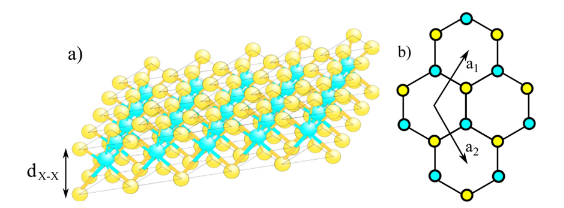
\includegraphics{tmdStructure.PNG}
    \caption{Structure of mono-layer TMD (a) side view (b) top view\cite{Andor}}
    \label{fig:my_label}
\end{figure}

The common sequence of steps followed in VASP simulations were, to use their "infomatica" material data base and search for the required material. The database gives out the available material systems within various space groups. To identify the most reliable system, we filter out the median of all the structures given, and use the one with the highest value. This ensures, to an extent, that the material parameters are reliable. The obtained material is generally in 2-3 layer format. We convert this structure to a monolayer by removing the the extra layers (literally deleting the atoms in VASP, a little strange idea, but the code behind it is strong enough to understand this "deletion", so does not give erroneous values). To further ensure that the repeated layer do not interact with each other, we increase the height lattice parameter ("c") to 20-30 A ("c" generally is about 12A). We used plane-wave cut off of 500-600 eV and optimization limit between 1e$^-5$ eV and 1e$^-3$ eV. 

For NEMO5 simulations for e-k, a similar approach was taken. Although, instead of mentioning the lattice constant "c" as 20-30 A, we designed the geometry and domain of the sample such that negligible interaction is seen between two consecutive layers. Here too, we first define the structure of the material, mention the tight binding parameter to be used for energy-band calculations and the value of lattice's atomic radii. Then the domain and geometry is decided, which, if domain is fixed at 1x1x1, a monolayer structure could be achieved.
The following section briefly describe the results obtained for each of the mentioned TMD materials, tool based tweaks performed, tight binding models used, k-space matrix used, and the band structure along the high symmetry points along with their respective energy gaps obtained from both the tools. 
\section{Molybdenum Disulfide (MoS2)}
Molybdenum disulfide's most explored space-group configuration is p63/mmc (in 3D) and P6mm in 2D. This configuration is the result of a hexagonal structure of the primitive lattice in 2 dimensional space with mirroring along 2 axis. 
\subsection{Crystal Structure and Band-Structure}
The crystal structure of MoS$_2$ is best visualized using the GUI provided by MedeA. The structure shows sp$^2$d$^5$ hybridization, therefore allowing strong covalent bonding between Molybdenum molecule and sulfur molecules. 
Using this structure, we bring the symmetry down to P1 (primitive cell) to convert the bulk structure to a monolayer using the steps mentioned above. Figure 4.2(a) and (b) show the before and after images of bulk to monolayer conversion. Before any calculations can be performed, we re-raised the symmetry of the system to p6m bringing it closest to a monolayer MoS$_2$. This way the brillouin zone of the material is conserved to zinc-blend. 

\begin{figure}
\centering
\begin{subfigure}{0.25\linewidth}
\centering
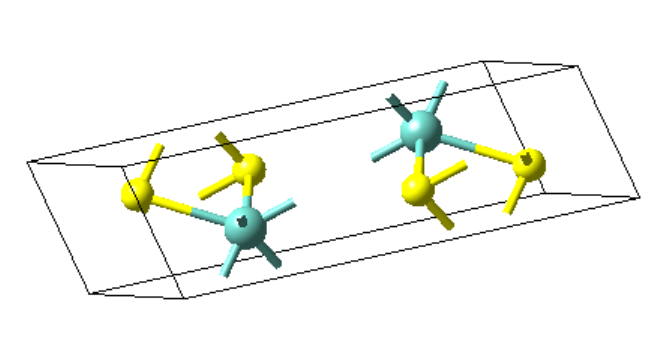
\includegraphics[width=\linewidth]{MoS2_VASP_bulk.PNG}
\caption{MoS$_2$ VASP bulk}
\label{fig:sub:left}
\end{subfigure}
\quad\quad\quad\quad
\begin{subfigure}{0.25\linewidth}
\centering
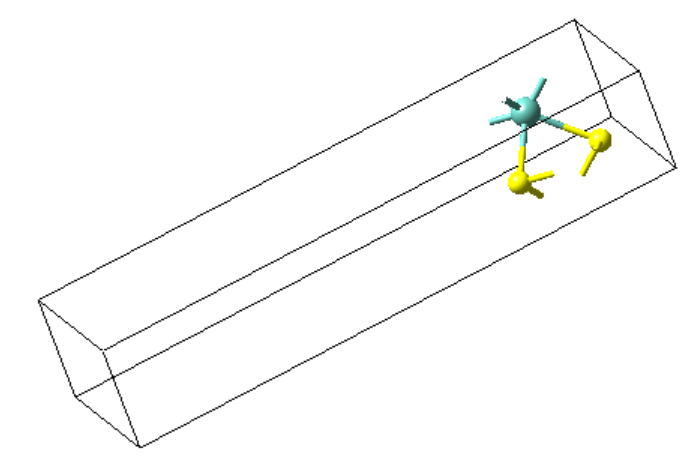
\includegraphics[width=\linewidth]{MoS2_VASP_mono.PNG}
\caption{MoS$_2$ VASP monolayer}
\label{fig:sub:right}
\end{subfigure}
\caption{Structure of MoS$_2$ (a) bulk, bilayer (b) monolayer, with lattice constant c = 20A}
\label{fig:sub}
\end{figure}

\subsection{VASP simulation}
We used MedeA-VASP to calculate e-k plots and Density of States for MoS$_2$. First step towards band-structure calculation was cell relaxation. This enabled a stress free structure for the crystal. Second step was to identify path of high symmetry points in Brillouin zone of MoS$_2$. Some literature quotes that monolayer of MoS$_2$ is a direct bandgap \textbf{[Give the refs here]}, but those study do not quote the  k-point at which this direct band-gap is found. First we took this as a discrepancy as we saw the system to show indirect bandgap at $\Gamma$-K k-point, the gap between minima found in Conduction band and maxima found in Valence band, but a direct band-gap was seen at K k-point. A few new literature \cite{Eugene,Gao} though clarifies this. Therefore, we follow the same k-point path for the band-structure study, i.e. $\Gamma$-M-K-Q-$\Gamma$. Study of Brillouin zone show the lack of band splitting at these given k-point path, therefore they are called points of high symmetry. This mentioned path is the most common calculation path used in studies and therefore, to calibrate VASP and NEMO, we used the same path as well.

Another aspect of e-k calculation is the k-space matrix. k-space matrix provides the simulator with the number of mesh points in the reciprocal space of the Brillouin zone. The effect of different k-space matrix is

\textbf{1.} Convergence of numerical models: for a dense mesh, a few failure in convergence points do not lead to incorrect results

\textbf{2.} Negative side, a denser matrix leads to high computational time.

For our simulations, a k-space matrix of 31x31x1, 7x7x1, and 20x4x1 were used. These matrices were used to replicate the system presented in literature for better comparison.

A final yet the most important aspect of electronic structure simulation of a material is the tight binding model used to calculate the values. For this experiment, we primarily relied on Density Functional Theory GGA-PBEsol. We 
Q which numerical model is used here? 
Q why? 
Q What about comparison to the rest?
Q. What is the expected bang gap, both with and without SOC? 
Q. What is the achieved band gap both with and without SOC?



\subsection{NEMO Simulations}
Ques to be answered for NEMO sim:
Q. How was the simulation different from that of VASP
Q. How were the results and their analysis different from VASP?
Q. What was the difference in the models used in nemo?
Q. is the k-space used in nemo and vasp the same? does it matter?
Q. Any comparison of nemo results to lit?


\begin{figure}
\centering
\begin{subfigure}{0.45\linewidth}
\centering
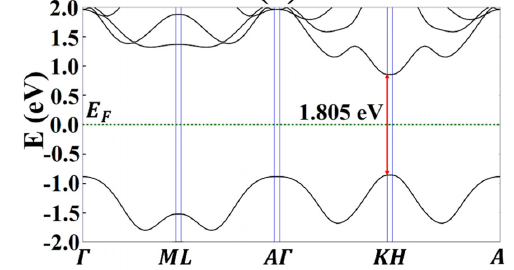
\includegraphics[width=\linewidth]{MoS2_DFT_lit.PNG}
\caption{MoS$_2$ VASP From Gao et.al \cite{Gao}}
\label{fig:sub:left}
\end{subfigure}
\quad\quad\quad\quad
\begin{subfigure}{0.4\linewidth}
\centering
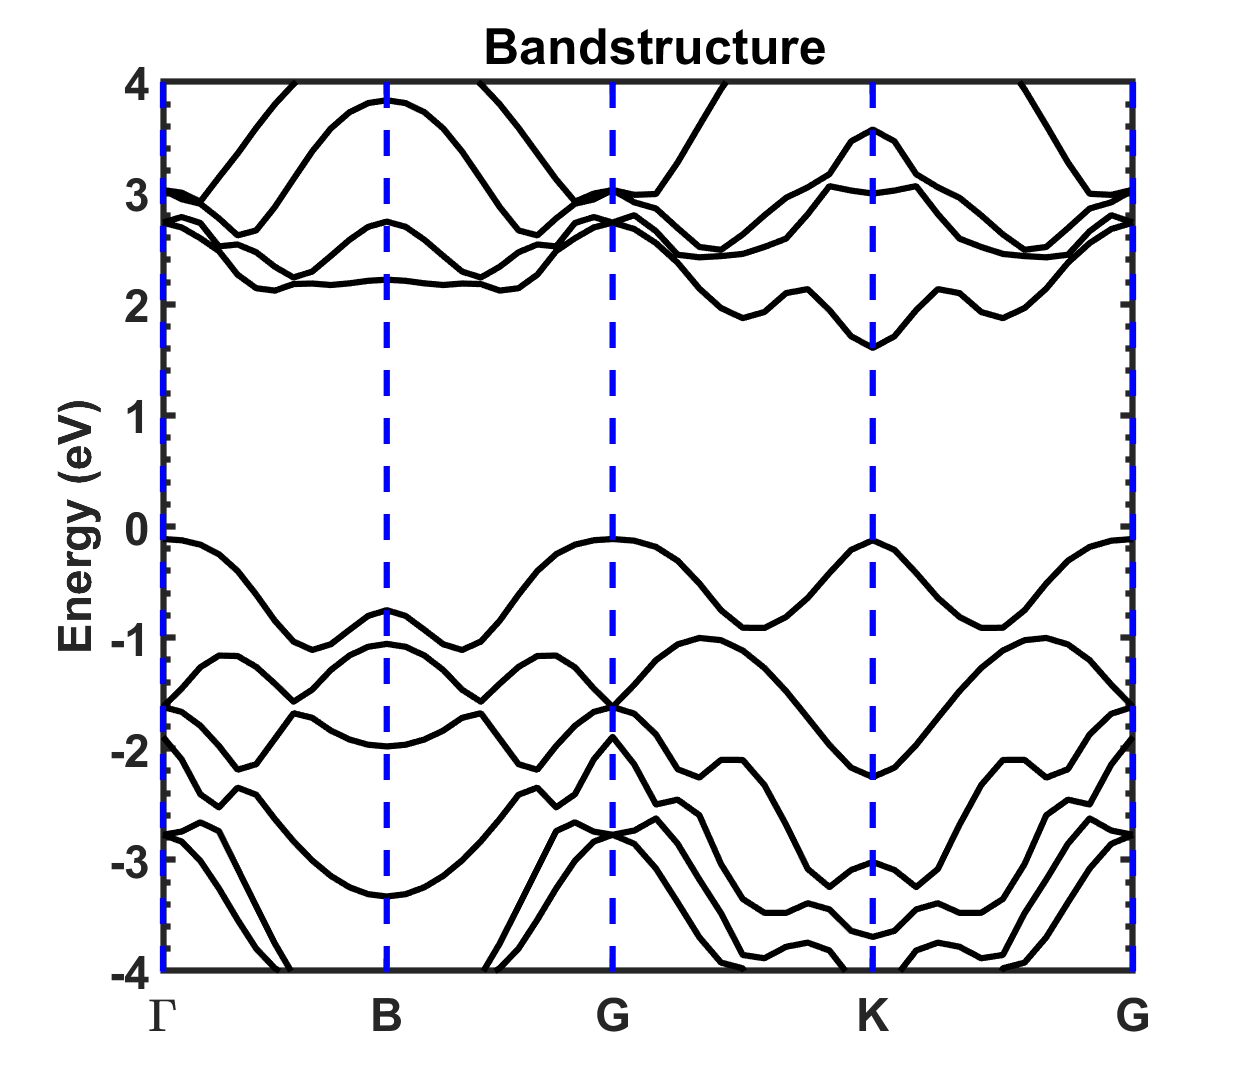
\includegraphics[width=\linewidth]{MoS2_DFT_sim.png}
\caption{MoS$_2$ VASP monolayer}
\label{fig:sub:right}
\end{subfigure}
\caption{Band structure comparison of simulation v/s literature \cite{Gao}}
\subcaption{The literature result shows a direct bandgap of 1.8 eV at K k-point }
\subcaption{(b) Using VASP and similar conditions as \cite{Gao}, the plot is re-created and is found in agreement with a direct bandgap at K k-point}
\label{fig:sub}
\end{figure}


\section{Tungsten Ditelluride (WTe2)}
\subsection{Crystal Structure}
\subsection{Band Structure}
\section{Molybdenum Diselunide (MoSe2)}
\subsection{Crystal Structure}
\subsection{Band Structure}
\section{Tungsten Disufide (WS2)}
\subsection{Crystal Structure}
\subsection{Band Structure}
\section{Conclusion}

\chapter{Device Simulations}
\section{Tunnel Diodes}
\subsection{Convergence Study}
\section{Tunnel Field Effect Transistors: NEMO study}
\subsection{Device's Structure in simulation}
\subsection{IV Curves}
\subsection{Test: Effect of Varying Channel Length}
\subsection{Test: DIBL in MoS2 TFET}
\section{Conclusion}

\chapter{Summary and Conclusion}

\chapter{Future Work}






%\lipsum{}

% Also include figures the normal way, using the graphicx package, or however
% you choose to do it
\begin{figure}
\centering

\includegraphics{kgcoelogohoriz}
\caption{Trust me, this is a figure}
\label{fig:samp}
\end{figure}

% A subfigure can be created using the environments provided in the subcaption
% package
\begin{figure}
\centering
\begin{subfigure}{0.25\linewidth}
\centering

\includegraphics[width=\linewidth]{kgcoelogovert}
\caption{Left subfigure}
\label{fig:sub:left}
\end{subfigure}
\quad\quad\quad\quad
\begin{subfigure}{0.25\linewidth}
\centering

\includegraphics[width=\linewidth]{kgcoelogovert}
\caption{Right subfigure}
\label{fig:sub:right}
\end{subfigure}
\caption{This is the caption for the entire figure}
\label{fig:sub}
\end{figure}

some more\footnote{aoeu} text

% Tables are unchanged as well
\begin{table}
\centering
\caption{Example of a table}
\label{tab:samp}
\begin{tabular}{cc}
\toprule
a		& b\\
\midrule
1		& 5\\
2		& 9\\
3		& 2\\
4		& 2\\
\bottomrule
\end{tabular}
\end{table}

% Citing some stuff
\nocite{cheung,zhao,cao,zhang}

% Citing everything
\nocite{*}

% Making the bibliography, using the IEEE format. By default the IEEE format
% won't replace author's names with et al., even when there are a lot of
% authors. Consult the IEEE LaTeX format documentation for how to change that,
% if desired.
\makebibliography{example}

% The theappendix environment is used when there is only one appendix.
% Otherwise use \appendix. Do not use both the theappendix environment
% and \appendix
\begin{theappendix}{Single appendix title}
	\section{stuff}
	\lipsum[15-21]
\end{theappendix}

% \appendix begins the appendicies. If you have just one appendix, it should
% technically be just "Appendix" not "Appendix A" and should be referred to in
% the text as "the appendix".
\appendix

% Begin a new appendix by starting new chapters
\chapter{Sample Appendix}

% You can make sections in appendicies, but I don't think many people will
\section{test section---probably not necessary}
\lipsum[6-12]
\chapter{Another Sample Appendix}
\lipsum[10-11]

% and finally, end the document
\end{document}
